\documentclass[tikz,border=8pt]{standalone}
\usepackage{tikz}
\usetikzlibrary{3d,calc,positioning}

\usepackage{tikz}
\usepackage{tkz-base}
\usetikzlibrary{quotes,angles}
\usetikzlibrary {arrows.meta}
%\usepackage{tkz-euclide}
\usetikzlibrary{calc}
\usetikzlibrary{shapes.geometric, shapes.misc, arrows}

\tikzstyle{startstop} = [rectangle, rounded corners, 
minimum width=3cm, 
minimum height=1cm,
text centered, 
draw=black]

\tikzstyle{io} = [trapezium, 
trapezium stretches=true, % A later addition
trapezium left angle=70, 
trapezium right angle=110, 
minimum width=3cm, 
minimum height=1cm, text centered, 
draw=black]

\tikzstyle{process} = [rectangle, 
minimum width=3cm, 
minimum height=1cm, 
text centered, 
text width=5cm, 
draw=black]

\tikzstyle{decision} = [diamond, 
minimum width=3cm, 
minimum height=1cm, 
text centered, 
draw=black]

\tikzstyle{startfor} = [chamfered rectangle, 
chamfered rectangle corners={north west, north east},
minimum width=3cm, 
minimum height=1cm, 
text centered, 
draw=black]

\tikzstyle{endfor} = [chamfered rectangle, 
chamfered rectangle corners={south west, south east},
minimum width=3cm, 
minimum height=1cm, 
text centered, 
draw=black]

\tikzstyle{block} = [style=draw, 
	minimum width = 1.6cm,
	minimum height = 1.2cm]
\tikzstyle{arrow} =[-{Latex[length=3mm]}, thick]

\newcommand{\drawsum}[2]{\node[draw,
	circle,
	minimum size=1cm
	] (#1) at #2{};
	\draw (#1.north east) -- (#1.south west)
	(#1.north west) -- (#1.south east)}

\newcommand{\fillsumsouth}[1]{\draw[fill=black] (#1.center) -- ++(-135:0.5cm) arc (-135:-45:0.5cm) -- cycle}
\newcommand{\fillsumnorth}[1]{\draw[fill=black] (#1.center) -- ++(135:0.5cm) arc (135:45:0.5cm) -- cycle}

\begin{document}
	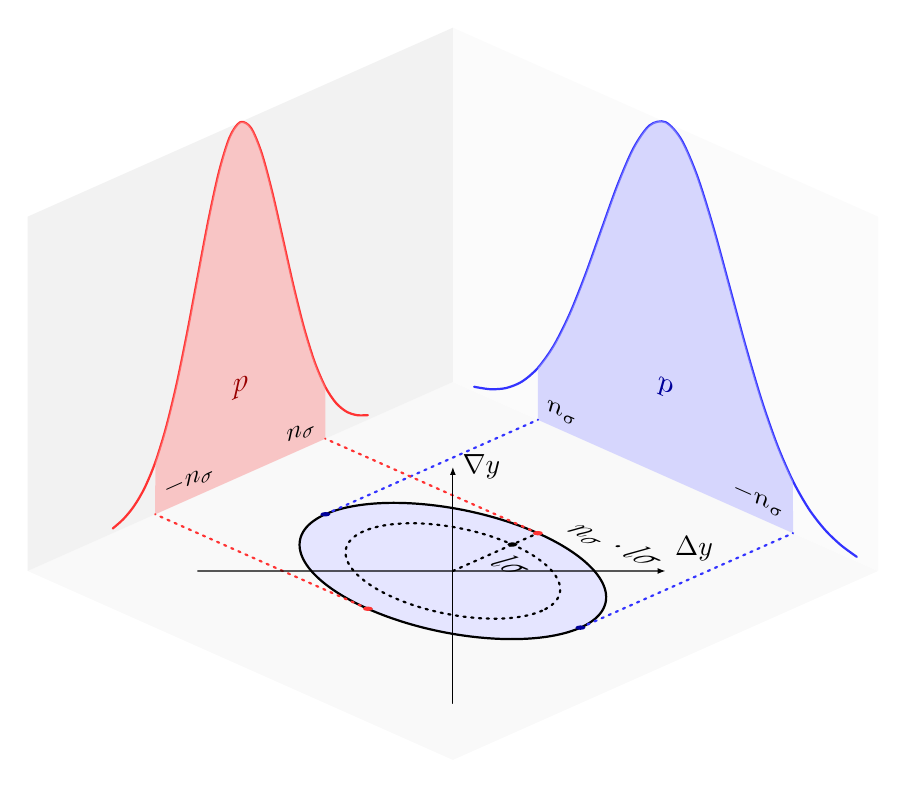
\begin{tikzpicture}[scale=3, line join=round, line cap=round,
		x={(0.9cm,-0.4cm)}, y={(-0.9cm,-0.4cm)}, z={(0cm,0.75cm)}] 
		% система координат выбрана для псевдоизометрии
		
		% параметры куба
		\def\a{2.0} % размер куба (ось OX, OY, OZ от 0 до a)
		\def\mu{1.0} % центр эллипса
		\def\rx{0.6} % полуось эллипса по X
		\def\ry{0.4} % полуось эллипса по Y
		\def\sx{0.6} % ширина 95% для X-плотности
		\def\sy{0.4} % ширина 95% для Y-плотности
		\def\sig{0.7}
		
		% ---- 1. Куб: только три задние грани ----
		% нижняя грань OXY
		\fill[gray!5] (0,0,0) -- (\a,0,0) -- (\a,\a,0) -- (0,\a,0) -- cycle;
		% задняя правая грань OXZ
		\fill[gray!3] (0,0,0) -- (\a,0,0) -- (\a,0,\a) -- (0,0,\a) -- cycle;
		% задняя левая грань OYZ
		\fill[gray!10] (0,0,0) -- (0,\a,0) -- (0,\a,\a) -- (0,0,\a) -- cycle;
		
		% ---- 2. Эллипс на нижней грани (OXY) ----
		\draw[thick,fill=blue!10]
		plot[domain=0:360,samples=200,variable=\t]
		({\mu+\rx*cos(\t)}, {\mu+\ry*sin(\t)}, 0);
		
		\draw[dotted, thick]
		plot [domain=0:360, samples=200, variable=\t]
		({\mu + \sig*\rx*cos(\t)}, {\mu + \sig*\ry*sin(\t)}, 0);
		
		% центр эллипса
		%\coordinate (C) at (\mu,\mu,0);
		%\fill (C) circle (0.3pt) node[below right=1pt] {$O'$};
		
		% ---- 3. График плотности X на задней правой грани (OXZ) ----
		% Форма нормального распределения (упрощённо как колокол)
		\draw[thick,blue!80]
		plot[domain=\mu-1.5*\sx:\mu+1.5*\sx,smooth,variable=\x]
		({\x},{0}, {2*exp(-((\x-\mu)^2)/(2*(\sx/1.96)^2))});
		
		% заполнение 95% области
		\fill[blue!30,opacity=0.5]
		plot[domain=\mu-\sx:\mu+\sx,smooth,variable=\x]
		({\x},{0},{2*exp(-((\x-\mu)^2)/(2*(\sx/1.96)^2))})
		-- (\mu+\sx,0,0) -- (\mu-\sx,0,0) -- cycle;
		
		% пунктир от эллипса к грани XZ
		\draw[blue!80, dotted,thick] ({\mu-\rx},\mu,0) -- ({\mu-\rx},0,0);
		\draw[blue!80, dotted,thick] ({\mu+\rx},\mu,0) -- ({\mu+\rx},0,0);
		
		\draw[dotted, thick] (\mu, \mu, 0) -- (\mu, {\mu - \ry}, 0);
		
		% ---- 4. График плотности Y на задней левой грани (OYZ) ----
		\draw[thick,red!80]
		plot[domain=\mu-1.5*\sy:\mu+1.5*\sy,smooth,variable=\y]
		({0},{\y},{2*exp(-((\y-\mu)^2)/(2*(\sy/1.96)^2))});
		
		% заполнение 95% области
		\fill[red!40,opacity=0.5]
		plot[domain=\mu-\sy:\mu+\sy,smooth,variable=\y]
		({0},{\y},{2*exp(-((\y-\mu)^2)/(2*(\sy/1.96)^2))})
		-- (0,\mu+\sy,0) -- (0,\mu-\sy,0) -- cycle;
		
		% пунктир от эллипса к грани YZ
		\draw[red!80, dotted,thick] (\mu,{\mu-\ry},0) -- (0,{\mu-\ry},0);
		\draw[red!80, dotted,thick] (\mu,{\mu+\ry},0) -- (0,{\mu+\ry},0);
		
		% ---- 5. Минимальные подписи ----
		%\node[below left] at (0,0,0) {$O$};
		%\node[right] at (\a,0,0) {$X$};
		%\node[above] at (0,\a,0) {$Y$};
		%\node[above right] at (0,0,\a) {$Z$};
		\begin{scope}[canvas is xz plane at y=0, transform shape]
			\node[blue!60!black, xscale=1, centered, yscale=1.2, scale=0.4] at (\mu,0.5) {$p$};
			\node[centered, yscale=1.2, scale=0.35, above left] at (\mu+\rx,0) {$-n_\sigma$};
			\node[centered, yscale=1.2, scale=0.35, above right] at (\mu-\rx,0) {$n_\sigma$};
		\end{scope}
		\begin{scope}[canvas is yz plane at x=0, transform shape]
			\node[red!60!black, centered, xscale=-1, yscale=1.2, scale=0.4] at (\mu,0.5) {$p$};
			\node[centered, xscale=-1, yscale=1.2, scale=0.35, above right] at (\mu+\ry,0) {$-n_\sigma$};
			\node[centered, xscale=-1, yscale=1.2, scale=0.35, above left] at (\mu-\ry,0) {$n_\sigma$};
		\end{scope}
		\begin{scope}[canvas is xy plane at z=0, transform shape]
			\node [circle, fill, scale=0.1] (sig) at (\mu, \mu - \sig*\ry) {};
			\node [red!80, circle, fill, scale=0.1] (nsig) at (\mu, \mu - \ry) {};
			\node [red!80, circle, fill, scale=0.1] at (\mu, \mu + \ry) {};
			\node [blue!60!black, circle, fill, scale=0.1] at (\mu + \rx, \mu) {};
			\node [blue!60!black, circle, fill, scale=0.1] at (\mu - \rx, \mu) {};
			
			\node [above right, yscale=-1.1, scale=0.4] at (nsig) {$n_\sigma \cdot l\sigma$};
			\node [below right, yscale=-1.1, scale=0.4] at (sig) {$l\sigma$};
			%\node[red!60!black, centered, xscale=-1, yscale=1.2, scale=0.4] at (\mu,0.5) {pvalue};
			%\node[centered, xscale=-1, yscale=1.2, scale=0.35, above right] at (\mu+\ry,0) {$-n_\sigma$};
			%\node[centered, xscale=-1, yscale=1.2, scale=0.35, above left] at (\mu-\ry,0) {$n_\sigma$};
		\end{scope}
		
			\draw [-{Latex[length=1mm]}] (\mu - 0.6, \mu + 0.6, 0) -- ({\mu + 0.5}, {\mu - 0.5}, 0) node [above right] {$\Delta y$};
			\draw [-{Latex[length=1mm]}] (\mu + 0.7, \mu + 0.7, 0) -- ({\mu - 0.55}, {\mu - 0.55}, 0) node [right] {$\nabla y$};
		
	\end{tikzpicture}
\end{document}
